\chapter{Stato dell'arte} %\label{1cap:spinta_laterale}
% [titolo ridotto se non ci dovesse stare] {titolo completo}
%

\begin{citazione}
    \textit{Lo scopo di questo capitolo è di illustrare la situazione attuale dei vari applicativi che sono a disposizione degli utenti del trasporto pubblico locale (TPL) per permettergli di organizzare i loro spostamenti. Nello specifico, viene preso in considerazione il caso di Moovit e della sua piattaforma di crowdsourcing di informazioni sulla mobilità in una determinata zona. Vengono inoltre sottolineate le similitudini e le differenze con \textsc{ShallWeGo}.}
\end{citazione}

\newpage

I principali attori sul panorama della diffusione di informazioni sul TPL sono senz'altro la piattaforma Maps di Google ed in particolare Moovit, che ha acquisito una maggiore popolarità nell'ultimo anno.

\section{Google Maps}
    \textbf{Transit} è un servizio messo a disposizione da Google ed integrato nella piattaforma Maps che consente all'utente di visualizzare le informazioni \textit{statiche} messe a disposizione dalle varie aziende di trasporto tramite il programma "Google Transit Partners", che consistono nella programmazione giornaliera delle corse e dell'organizzazione delle fermate sul territorio in questione. \\
    Oltre ai dati statici, le aziende di trasporto possono condividere con Google mediante la piattaforma \textbf{Realtime Transit}, che permette di visualizzare all'interno di Maps i dati in tempo reale sulla posizione dei mezzi pubblici in un determinato istante. Questa funzionalità, così come tutti i dati relativi al trasporto pubblico su Maps sono disponibili solo su iniziativa delle aziende che decidono di partecipare al programma. Un esempio di azienda che mette a disposizione i dati realtime è per esempio l'ATAC di Roma, che li offre a partire da Settembre 2019 (\cite{atactransit})  \\
    I dati (siano essi statici o dinamici) sono comunicati a Google su base regolare dalle aziende (tipicamente settimanale, secondo quanto riportato nella sezione FAQ della pagina dedicata \footnote[3]{\url{https://developers.google.com/transit/gtfs/guides/faq}}) tramite il formato GTFS \textit{(General Transit Feed Specification)} che permette di strutturare in maniera efficiente i dati riguardanti il trasporto pubblico.

    Esistono due "varianti" del formato GTFS:
    \begin{itemize}
        \item \textbf{GTFS Statico}, che raccoglie i dati "statici" (quindi gli orari previsti delle corse e l'organizzazione delle fermate sul territorio);
        \item \textbf{GTFS Realtime}, che raccoglie i dati "dinamici" (come l'andamento delle corse in tempo reale)
    \end{itemize}

    Tuttavia, come accennato in precedenza, questi dati sono comunicati su richiesta delle aziende e solo un numero limitato di queste ultime (almeno in Italia) aderisce al programma, limitando così i dati a disposizione dell'utente.

\section{Mobilità e crowdsourcing}
    La tecnica del crowdsourcing, applicabile nella maggior parte dei casi in cui ci sia bisogno di ottenere dati di interesse per un determinato dominio consiste nel ricavare direttamente questi ultimi da persone sul campo e che ritengano di possedere un'informazione che potrebbe tornare utile alla comunità.
    Anche nel caso della piattaforma che si vuole sviluppare, è possibile andare ad isolare i dati di interesse (quelli utili cioè a fornire un sufficiente livello di informazione agli utenti del TPL). Possono essere riassunti in cinque punti:
            \begin{itemize}
                \item Posizione di una fermata in un determinato punto;
                \item "Equipaggiamento" di una fermata (in termini di pensilina, segnali identificativi e quadri orari disponibili al pubblico);
                \item Utilizzo di una fermata da parte di una determinata linea.
                \item Destinazioni di una linea;
                \item Eventi temporanei (come presenza di traffico, avvisi su deviazioni o strade chiuse);
            \end{itemize}

        L'approccio del crowdsourcing è già utilizzato in particolare da un'altra piattaforma che risulta di particolare interesse, ovvero \textbf{Moovit}. Essa ne fa uso per ottenere dati riguardanti aziende di trasporto che non vengono resi disponibili pubblicamente.

    \subsection{La Community di Moovit: un caso di studio}
        Moovit è una piattaforma che al contrario di Google Maps si occupa esclusivamente di mobilità.
        Nasce nel 2012 e nel 2015 viene acquistata da Intel. Attualmente Moovit si sta impegnando per sviluppare soluzioni di \textbf{Mobility as a Service}.
        Il Mobility as a Service (MaaS) è un concetto relativamente nuovo, che permette all'utente di scegliere il modo che ritiene più adatto di spostarsi (tramite mezzi pubblici, car sharing e simili) usando una sola piattaforma che mette a disposizione tutti questi servizi, favorendo quindi l'interoperabilità tra i vari mezzi di trasporto. \\

        Dal 2015, inoltre, Moovit mette a disposizione un servizio chiamato \textbf{Mooviters' Community}, che permette al singolo utente della piattaforma di partecipare alla mappatura delle fermate e delle linee della sua zona tramite un Editor accessibile via web. I cambiamenti dovranno quindi essere approvati dagli amministratori della piattaforma o da utenti esperti. \\

        In particolare, la piattaforma di Moovit organizza gli utenti in "livelli", che potranno essere "scalati" man mano che si matura esperienza in termini di numero di segnalazioni effettuate. Nello specifico, se un utente $x$ di livello $n$ effettua una segnalazione, coloro che potranno poi verificarla questa saranno solamente utenti $z$ il cui livello risulta almeno $n + 1$ o che siano membro del Team. \\
        Il problema di questo approccio è che se un utente con molta esperienza si unisce alla piattaforma in un certo momento, non potrà immediatamente cominciare a verificare segnalazioni a causa del suo livello troppo basso.\\
        Attualmente, l'Editor della Community di Moovit è disponibile in tutte le sue funzionalità esclusivamente via web tramite un browser che riporta uno \textit{user-agent} desktop. \\

        Oltre all'editor delle fermate e delle linee, nell'ultimo periodo Moovit ha messo a disposizione direttamente dalla sua applicazione mobile uno strumento che permette di segnalare anche l'affollamento di una determinata corsa, come riportato sul sito web della piattaforma.\footnote[4]{\url{https://moovit.com/press-releases/moovit-crowding-report/}}

        \begin{figure}[H]
            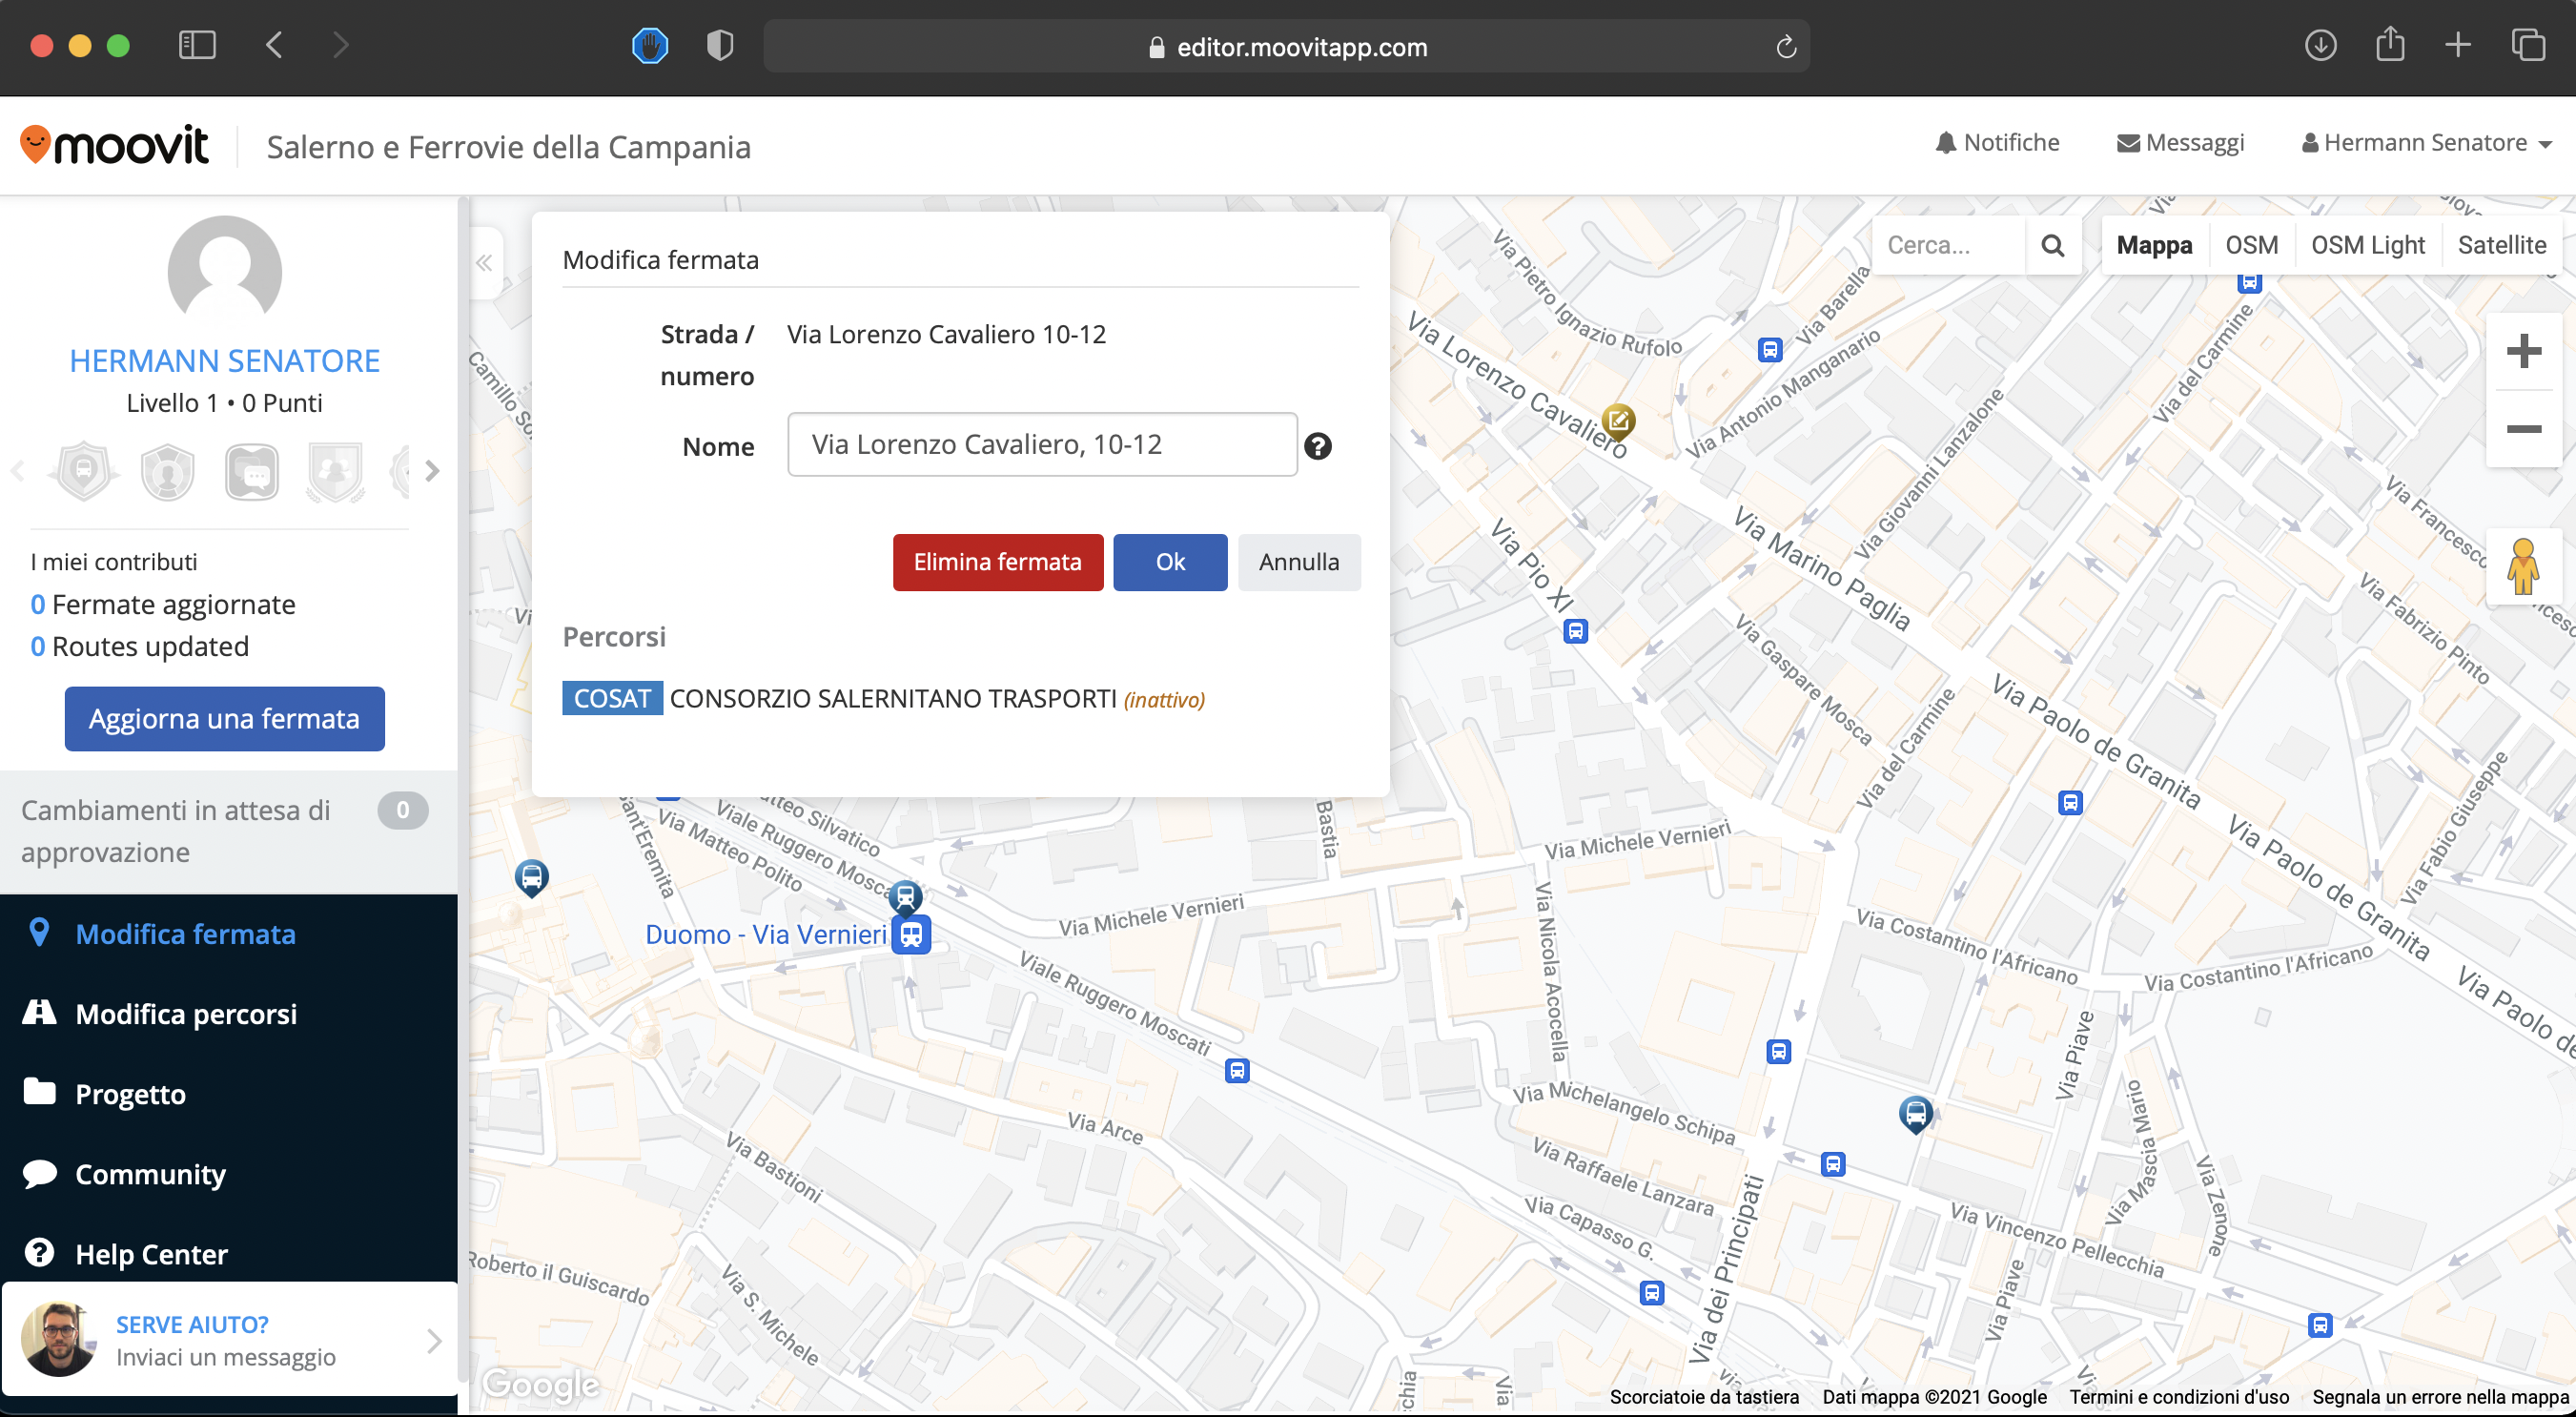
\includegraphics[width=\columnwidth]{capitolo2/figure/modificaFermata.png}
            \caption{Modifica di una fermata nella piattaforma di Moovit}
            \label{Modifica di una fermata nella piattaforma di Moovit}
        \end{figure}

        \begin{figure}[H]
            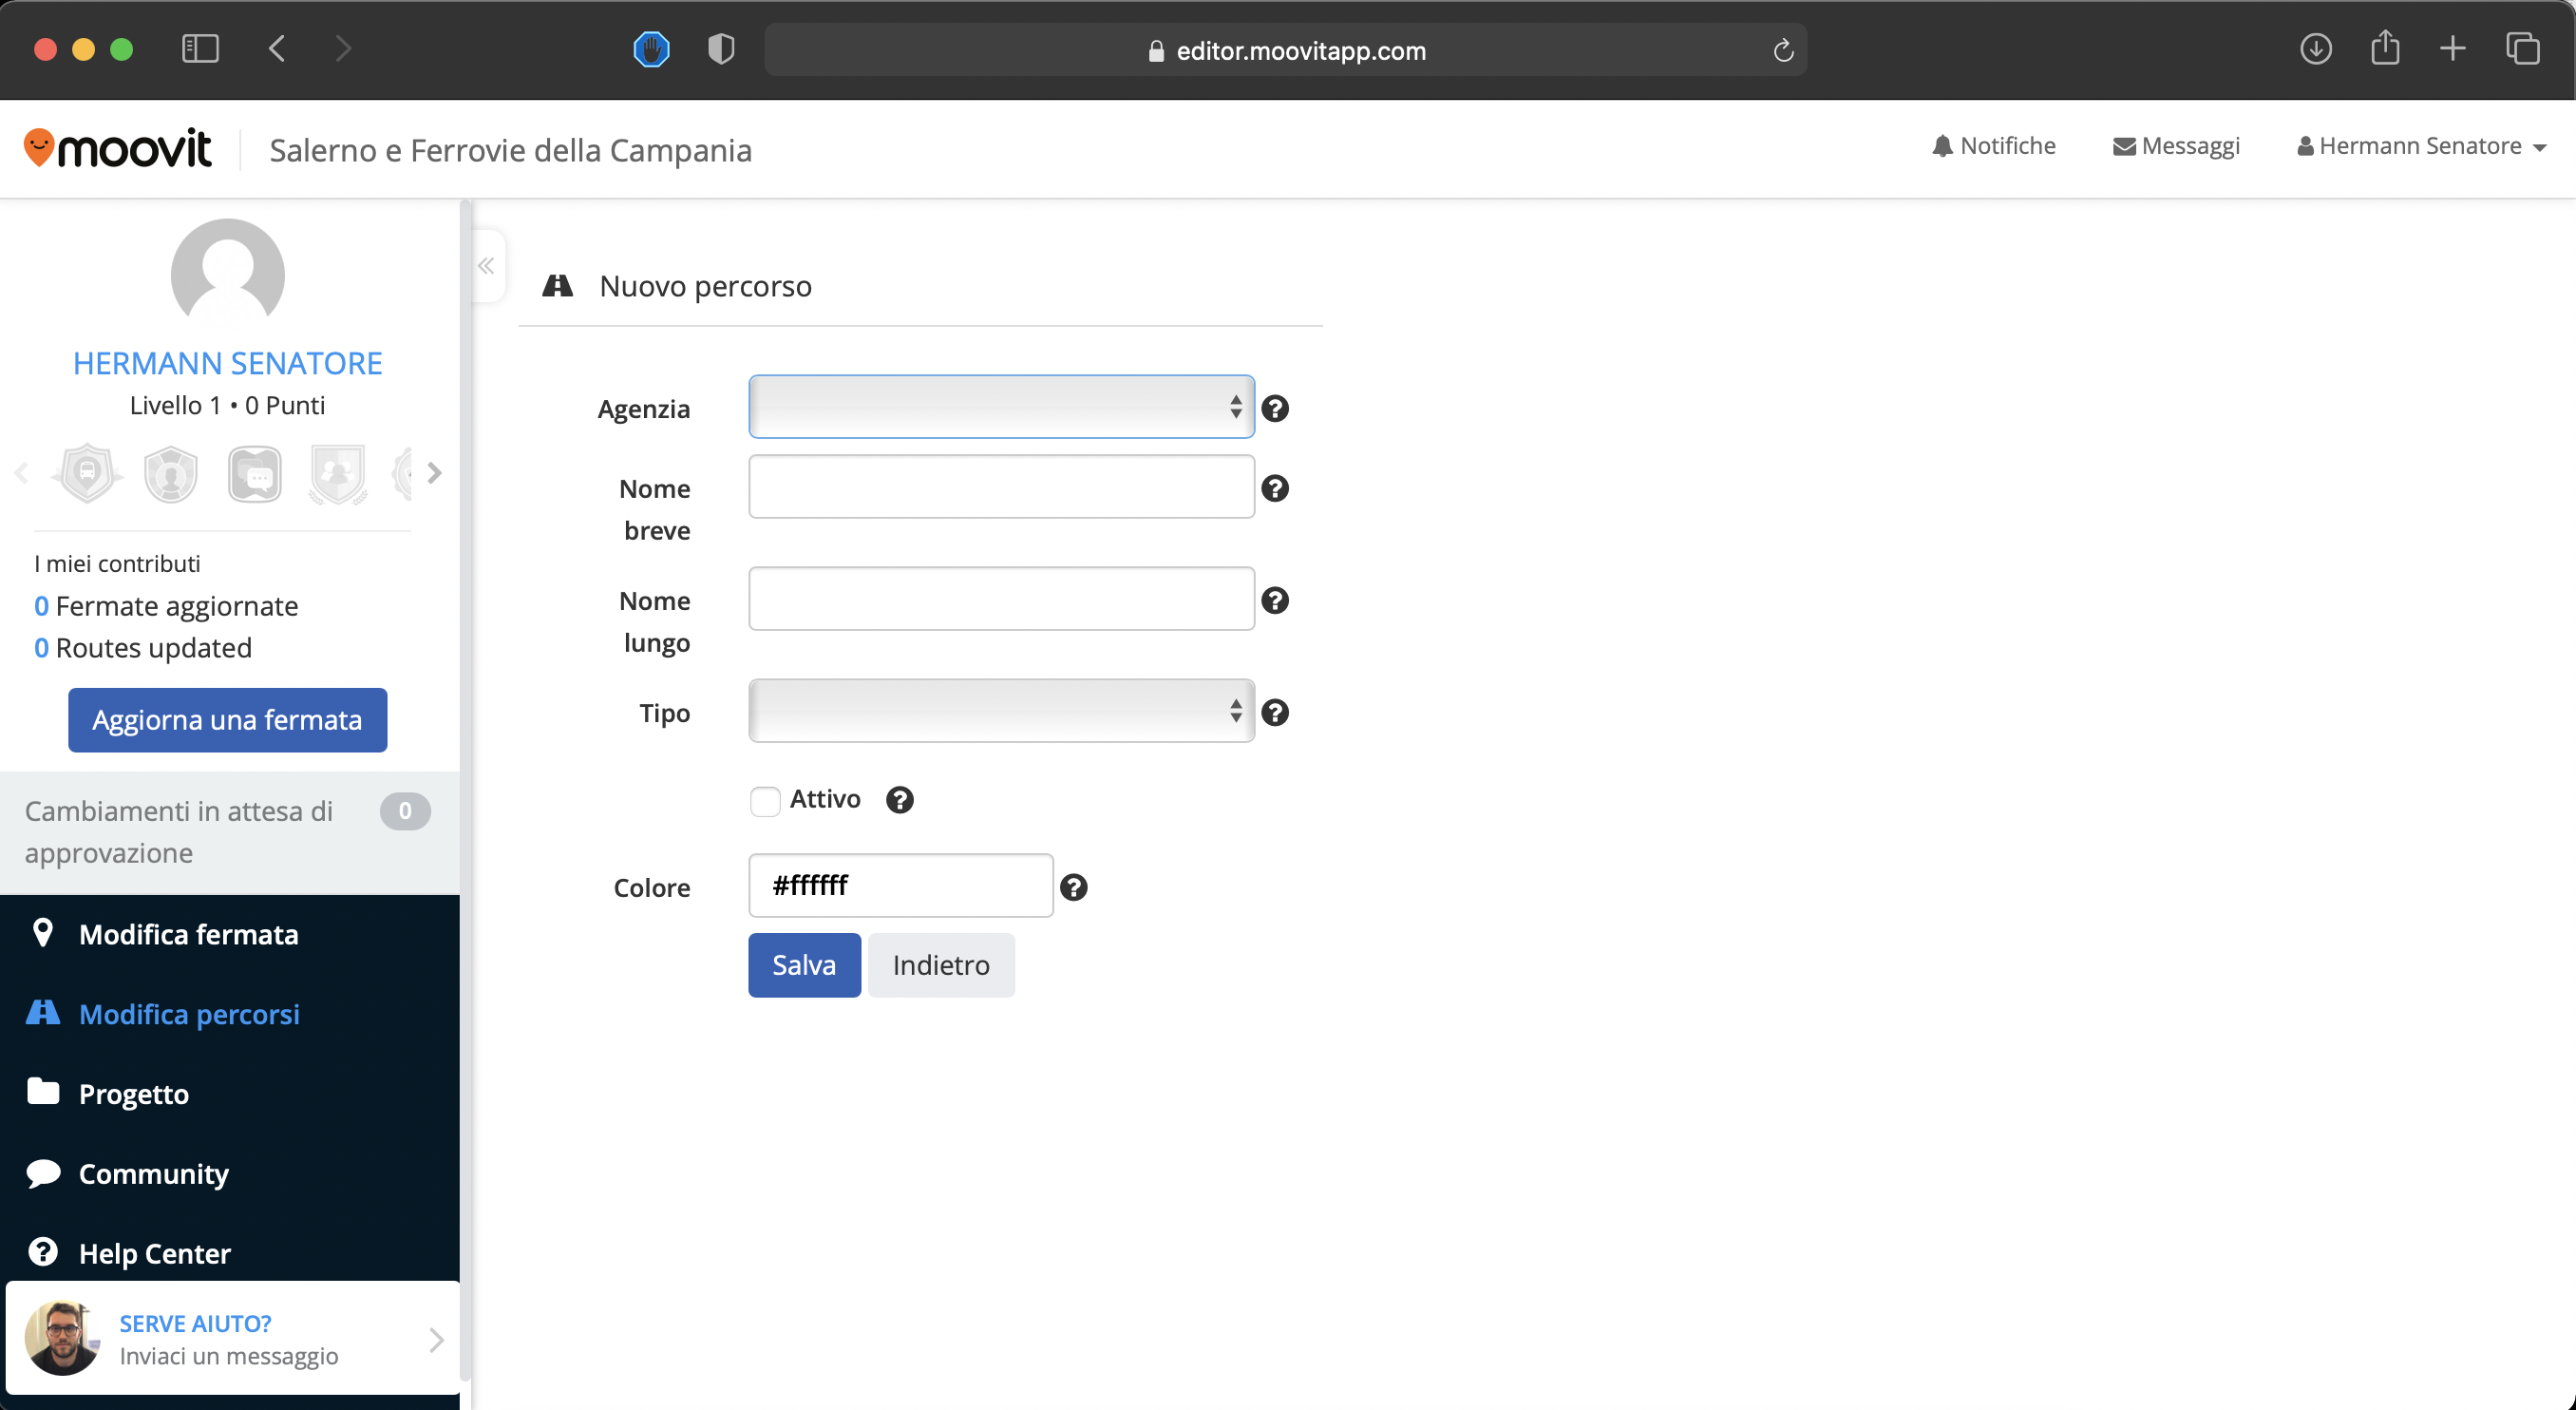
\includegraphics[width=\columnwidth]{capitolo2/figure/nuovoPercorso.png}
            \caption{Segnalazione di una fermata nella piattaforma di Moovit}
            \label{Segnalazione di una fermata nella piattaforma di Moovit}
        \end{figure}

        \begin{figure}[H]
            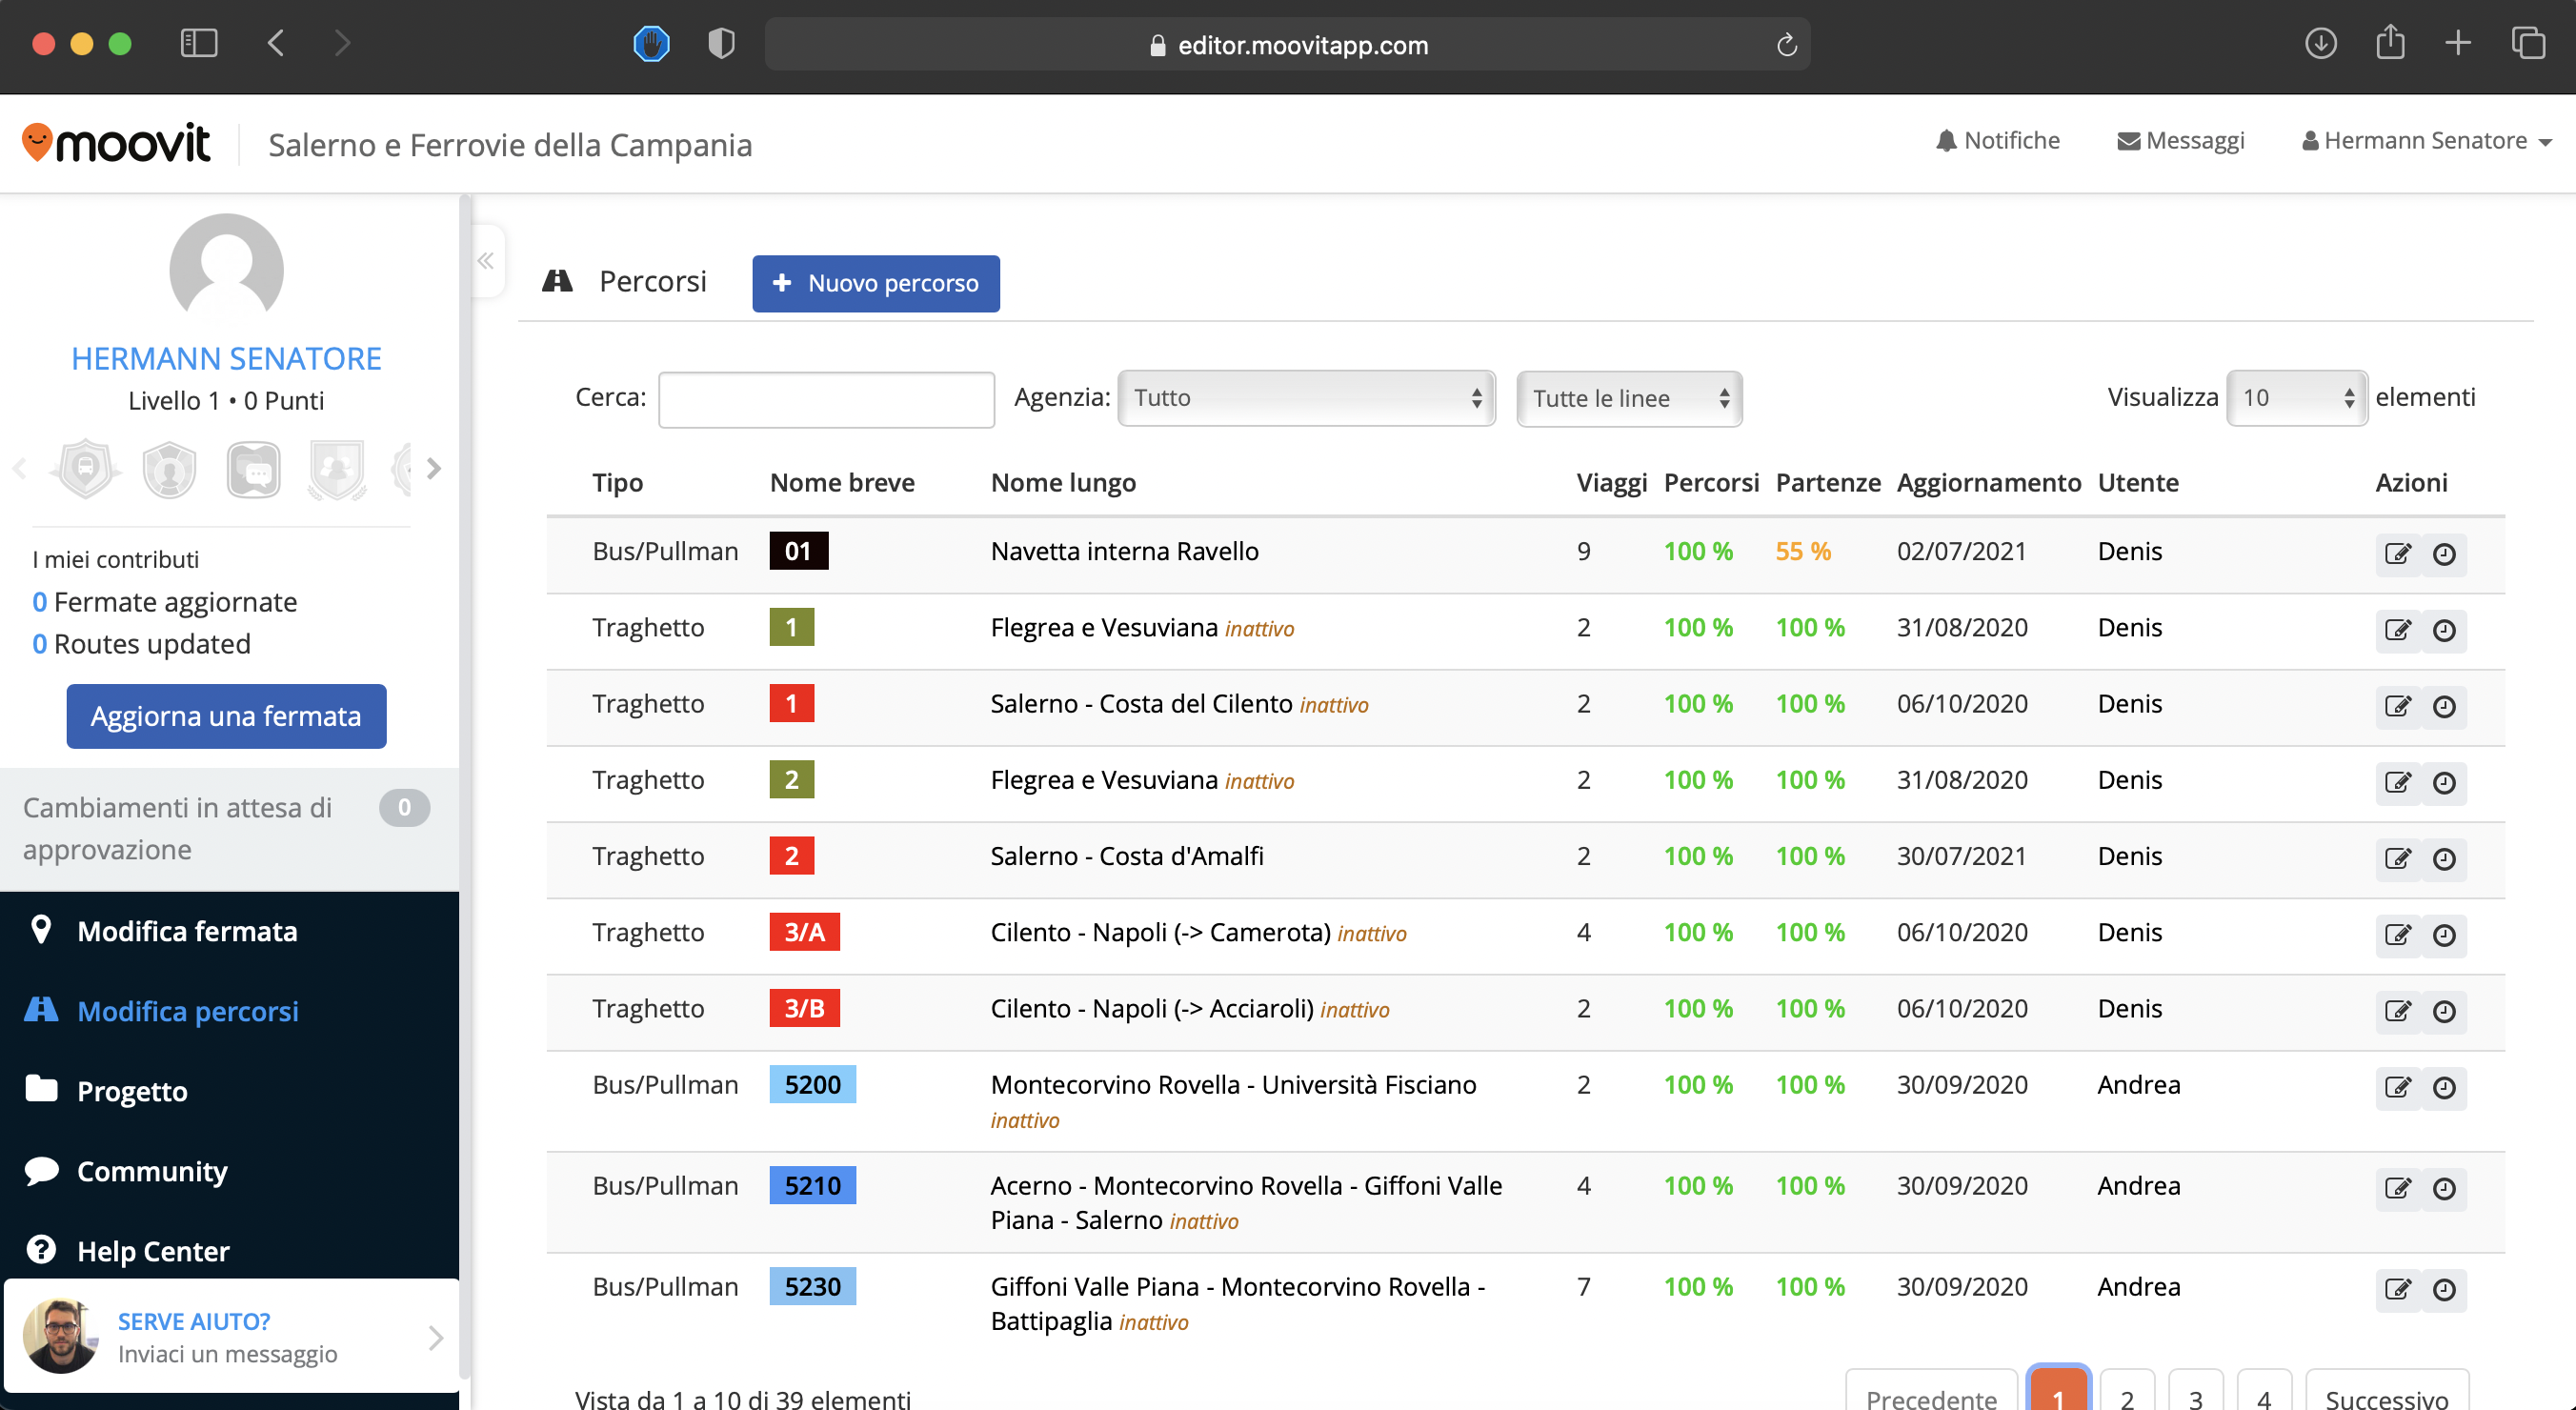
\includegraphics[width=\columnwidth]{capitolo2/figure/tuttiPercorsi.png}
            \caption{Linee segnalate dagli utenti sulla piattaforma di Moovit}
            \label{Linee segnalate dagli utenti sulla piattaforma di Moovit}
        \end{figure}

        

\newpage
\section{Il focus di \textsc{ShallWeGo}}
    La piattaforma \textsc{ShallWeGo} si basa principalmente sul modello delineato da Moovit con la sua Community rendendo tuttavia i dati ottenuti direttamente dagli utenti la fonte principale di informazione, fornendo gli strumenti adatti per rendere disponibili i dettagli sulle aziende, sulle corse e sulle fermate in una determinata zona tramite un'applicazione mobile che ne semplifichi l'accessibilità anche all'esterno in quanto, come accennato in precedenza, la piattaforma di Moovit risulta principalmente web-based, \textbf{separata dall'applicazione principale che è più conosciuta al grande pubblico.} \\
    Inoltre, a differenza della Community di Moovit, in \textsc{ShallWeGo} le segnalazioni non sono limitate solamente a dettagli statici ma si estendono anche ad eventi "dinamici" (come strade chiuse, deviazioni, traffico o incidenti), ai dettagli di una singola fermata (come l'affollamento, la presenza di pensiline, di paline di riconoscimento delle aziende che la utilizzano o dei quadri orari) ed all'andamento delle corse, sfruttando il dispositivo dell'utente, permettendo quindi ad altri membri della community di verificare la presenza e la posizione di una corsa nell'ambito di una linea, in modo simile a quanto avviene con Transit Realtime di Google, ma con la differenza che non risulta necessario che le aziende condividano i dati. La feature presente in \textsc{ShallWeGo} permette anche di condividere informazioni sulla corsa stessa quali l'affollamento, la temperatura o le condizioni del mezzo in quel momento (come ad esempio lo stato di funzionamento delle obliteratrici o dell'aria condizionata) \\
    Dal punto di vista della verifica delle segnalazioni, \textsc{ShallWeGo} non possiede un team che si dedica a valutare le segnalazioni, ma al contrario i verificatori più adatti vengono scelti mediante una componente di Intelligenza Artificiale creata proprio a questo scopo ed integrata nell'infrastruttura dell'applicazione. In particolare, l'Algoritmo per la scelta degli utenti si basa, oltre che sull'esperienza accumulata sulla piattaforma da parte di un singolo (in termini di segnalazioni effettuate e valutate), anche sulla distanza geografica dell'area in cui egli opera dal luogo della segnalazione. In questo modo, anche i nuovi iscritti alla piattaforma avranno la possibilità di valutare le segnalazioni inviate alla piattaforma. I dettagli sul funzionamento della componente di Intelligenza Artificiale saranno discussi nel capitolo successivo. Infine, dal punto di vista implementativo, non è chiaro quante e quali tecnologie sono utilizzate dalla piattaforma di Moovit, dal momento che il codice sorgente di quest'ultima non sembra essere reperibile.